\section*{04/10}
	
		\begin{center}
		\textbf{Одномерные краевые элементы}
	\end{center}
	
	
	\begin{enumerate}
		\item Граничные условия Дирихле (I рода)
		\[
		u(0)=u_0, \ u(l)=u_l
		\]
		\item Граничные условия Неймана
		\[
		k(0)u'(0)=-\sigma_0; \quad k(l)u'(l)=\sigma_l; \quad -(ku')'=f
		\]
		\[
		u'=-\frac{1}{k}\int\limits_0^lfdx+C_1 \Rightarrow u=\int\limits_0^l (-\frac{1}{k}\int\limits_0^lfdx+C_1)dx+C_2 \Rightarrow u=u(x)+\overline{C_0}
		\]
		\[
		u(x_0)=C_0
		\]
	\end{enumerate}
	\underline{\hspace{3cm}}
	
	\[
		\int_{x_i}^{x_{i+1}} \delta q^T \left\{ \left[ B^T k B + N^T c B + \mathbf{N'}^T b N \right] q - N^T f \right\}   dx 
	\]
	\[
		N = \begin{bmatrix} N_1^{(i)},  N_2^{(i)} \end{bmatrix}; \quad
		N_1^{(i)} = 1 - \frac{x - x_i}{l_i}; \ N_2^{(i)} = 1 - \frac{x - x_i}{l_i} 
	\]
	\[
		B = \begin{bmatrix} B_1^{(i)},  B_2^{(i)} \end{bmatrix} = \begin{bmatrix} -\frac{1}{l_i},  \frac{\lambda}{l_i} \end{bmatrix}; \qquad
		\xi = x - x_i, \ d\xi = dx
	\]
	\[
		\int_0^{l_i} \left[ B^T k(x)B + N^T c(x) B + N^T b(x) N \right] d\xi
	\]
	\[
	\int\limits_0^{l_i} c(\xi+x_i) \begin{bmatrix}
		1-\frac{\xi}{l_i} \\ \frac{\xi}{l_i} 
	\end{bmatrix} \begin{bmatrix}
	-\frac{1}{l_i} & \frac{1}{l_i}
	\end{bmatrix} d\xi= \int\limits_0^{l_i} \frac{c(\xi+x_i)}{l_i} \begin{bmatrix}
	\frac{\xi}{l_i} - 1 & 1 - \frac{\xi}{l_i} \\
	-\frac{\xi}{l_i} & \frac{\xi}{l_i}
	\end{bmatrix} d\xi
	\]
	\newpage
	\begin{center}
		\textbf{Задача теплопроводности в стержне}
	\end{center}
	
	\begin{center}
	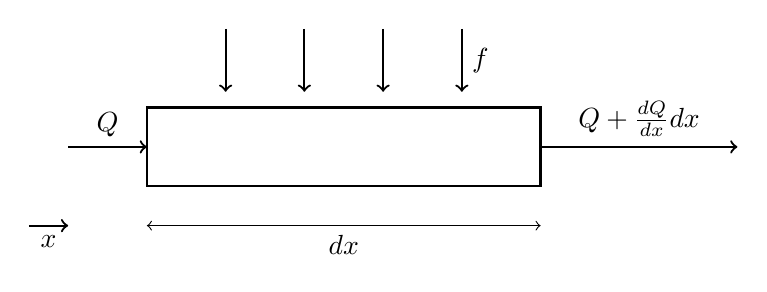
\begin{tikzpicture}
		
		% Draw the rectangle
		\draw[thick] (0,0) rectangle (5,1);
		
		% Arrows going into the rectangle with labels "f"
		\draw[->, thick] (1, 2) -- (1, 1.2);
		\draw[->, thick] (2, 2) -- (2, 1.2);
		\draw[->, thick] (3, 2) -- (3, 1.2);
		\draw[->, thick] (4, 2) -- (4, 1.2) node[midway, right] {$f$};
		
		% Label for dx
		\draw[<->] (0,-0.5) -- (5,-0.5) node[midway, below] {$dx$};
		
		% Label for Q on the left
		\draw[->, thick] (-1,0.5) -- (0,0.5) node[midway, above] {$Q$};
		
		% Label for Q+dQ/dx*dx on the right
		\draw[->, thick] (5,0.5) -- (7.5,0.5) node[midway, above] {$Q + \frac{dQ}{dx}dx$};
		
		% Arrow for x-axis direction
		\draw[->, thick] (-1.5,-0.5) -- (-1,-0.5) node[midway, below] {$x$};
		
	\end{tikzpicture}
	\end{center}
	
	\begin{equation}
		Q+fdx=Q+\frac{dQ}{dx}\cdot dx \Rightarrow f=\frac{dQ}{dx}
	\end{equation}
	
	\begin{equation}
		Q= -K_x \cdot \frac{dT}{dx} - \text{ закон Фурье}
	\end{equation}
	
	где $K_x=\lambda S$ - коэф. теплопроводности стержня, $\lambda$ - коэф. теплопроводности материала, 	$S$ - площадь сечения стержня.
	
	(2) $\rightarrow$ (1):
	\begin{equation}
	-\frac{d}{dx}(K_x \cdot \frac{dT}{dx}) = f
	\end{equation}
	
	\underline{Граничные условия:}
	\begin{enumerate}
		\item $T(0)=T_0, \ T(l)=T_l$
		\item $-K_x \cdot \dfrac{dT}{dx} |_{x=0} = q, \ -K_x \cdot \dfrac{dT}{dx} |_{x=l} = -q$
		\item $K_x \cdot  \dfrac{dT}{dx} |_{x=0} = -\alpha g (T_0 - T(0)), \ K_x \cdot \dfrac{dT}{dx} |_{x=l} = \alpha g (T_l - T(l))$
	\end{enumerate}
	
	\begin{center}
	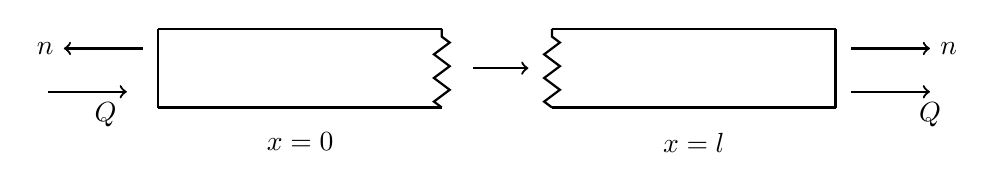
\begin{tikzpicture}
    % Левый конец стержня
    \draw[thick] (0.2,0) -- (3.8,0);
    \draw[thick] (0.2,1) -- (3.8,1);
    \draw[thick] (0.2,0) -- (0.2,1);
    \draw[thick, decorate, decoration={zigzag, segment length=3mm, amplitude=1mm}] (3.8,0) -- (3.8,1);

    % Правый конец стержня
    \draw[thick] (5.2,0) -- (8.8,0);
    \draw[thick] (5.2,1) -- (8.8,1);
    \draw[thick] (8.8,0) -- (8.8,1);
    \draw[thick, decorate, decoration={zigzag, segment length=3mm, amplitude=1mm}] (5.2,0) -- (5.2,1);
    
    % Силы
    \draw[->, thick] (0,0.75) -- (-1,0.75) node[left] { $n$};
    \draw[->, thick] (-1.2,0.2) -- (-0.2,0.2) node[below left] { $Q$};
    \draw[->, thick] (9,0.75) -- (10,0.75) node[right] { $n$};
    \draw[->, thick] (9,0.2) -- (10,0.2) node[below] { $Q$};

    % Обозначения координат
    \node[below] at (2,-0.2) { $x=0$};
    \node[below] at (7,-0.2) { $x=l$};
    
    \draw[->, thick] (4.2, 0.5) -- (4.9, 0.5);

\end{tikzpicture}
\end{center}
	
	Чтобы определить знак в граничных условиях второго рода нужно смотреть на направление $Q=K_x \cdot  \dfrac{dT}{dx}$.
	
	\underline{Интегральная формулировка:} $ \ r=-\dfrac{d}{dx}(K_x \cdot \dfrac{dT}{dx}) - f = 0, \quad v = \delta T $
	\begin{equation}
	\int\limits_0^l (-\frac{d}{dx}(K_x \cdot \frac{dT}{dx}) - f) \cdot \delta T \cdot S dx = 0 \Rightarrow \int\limits_0^l  \frac{d\delta T}{dx}(K_x \cdot \frac{dT}{dx}) \cdot S dx - F(\delta T) = 0
	\end{equation}
	\[
	 F(\delta T) = S(K_x \cdot \frac{dT}{dx})\cdot \delta T |_0^l = -SQ_l \cdot \delta T(l) + SQ_0 \cdot\delta T(0)
	 \]
	 \[  Q_0 = -K_x \cdot \frac{dT}{dx} |_{x=0}, Q_l = -K_x \cdot \frac{dT}{dx} |_{x=l}
	\]
	\[
	T= Nq = N_1^{(i)}T_i +  N_2^{(i)}T_{i+1}, \quad \frac{dT}{dx}=Bq
	\]
	\[ 	\delta T= N\delta q = N_1^{(i)}\delta T_i +  N_2^{(i)}\delta T_{i+1}, \quad \frac{d\delta T}{dx}=B\delta q
	\]
	
	\underline{Вариационная формулировка:}
	\[
		J(t) = \frac{1}{2} \int\limits_0^{l} K_x \left( \frac{dT}{dx} \right)^2 S \, dx - \int\limits_0^{l} SfT \ dx + S Q_l T_l - S Q_0 T_0 \rightarrow \min \quad \text{(совпадает с (4))} 
	\]
	\[
		\Delta J = J(T + \delta T) - J(T) = \frac{1}{2} \int\limits_0^{l} K_x S \left( \frac{d(T + \delta T)}{dx} \right)^2 dx - \int_0^{l} S f (T + \delta T) \, dx -
	\]
	\[  
		 \frac{1}{2} \int\limits_0^{l} K_x \left( \frac{dT}{dx} \right)^2 S \, dx +
		 \int\limits_0^{l} S f T \, dx + S Q_l (T_l + \delta T_l) - S Q_0 (T_0 -\delta T_0) -
		 S Q_l T_l + S Q_0 T_0 =
	\] 
	\[
		= \frac{1}{2} \int\limits_0^{l} S K_x \left[ \left( \frac{dT}{dx} \right)^2 + 2 \cdot \frac{dT}{dx} \cdot \frac{d \delta T}{dx} + \left( \frac{d \delta T}{dx} \right)^2 \right] dx - \int\limits_0^{l} S f \delta T \, dx -
	\]
	\[ \frac{1}{2} \int\limits_0^{l} S K_x \left( \frac{dT}{dx} \right)^2 dx + S Q_l \delta T_l - S Q_0 \delta T_0 
	\]
	
	Оставим линейную часть приращений $\Delta J$ относительно $\delta T$:
	\[
		\int\limits_0^{l} S K_x \frac{dT}{dx}\cdot \frac{d \delta T}{dx} \, dx - \int\limits_0^{l} S f \delta T \, dx + S Q_l \delta T_l - S Q_0 \delta T_0 \rightarrow (4)
	\]